%TODO:


\documentclass{scrartcl}


\usepackage[utf8]{inputenc}
\usepackage[english]{babel}
\usepackage{lmodern} 
\usepackage[T1]{fontenc}
\usepackage{booktabs}
\usepackage{multirow}
\usepackage{wrapfig}


% PAKETE
\usepackage{siunitx}
\usepackage{graphicx}
\usepackage[usenames,dvipsnames]{xcolor}
\usepackage{placeins}
\usepackage{longtable}
\usepackage{enumitem}
\usepackage{bbm}

\usepackage{amssymb} % math symbols
\usepackage{amsmath} % ams
\usepackage{amsfonts} % mathmatical fonts

% caption indenting
 \usepackage[format=plain,indention=0em,labelfont=bf,margin=1em]{caption} 
 \usepackage{subfig} %subfigures ^^
\usepackage[protrusion=true,expansion=true]{microtype} % denser font, "-" behind line
\usepackage{esint} % nicer double and triple integrals
\usepackage{fancyhdr} % fancy headers
\usepackage[colorlinks=true,linkcolor=black,citecolor=black,filecolor=black,urlcolor=black]{hyperref}



% EINSTELLUNGEN
\sisetup{seperr,repeatunits=false}
\numberwithin{equation}{section}
\numberwithin{figure}{section}
\numberwithin{table}{section}

% EIGENE FUNKTIONEN
\newcommand{\re}{\operatorname{Re}}
\newcommand{\im}{\operatorname{Im}}
\newcommand{\gquote}[1]{\glqq #1 \grqq}

\newcommand{\eq}[2]{\begin{equation}#1\label{#2}\end{equation}}
\newcommand{\eqand}[0]{\hspace{.25cm} \bigwedge \hspace{.25cm}}
\newcommand{\grafik}[2]{\begin{figure}[h]\centering \includegraphics[width=10cm]{#1.eps}  \caption{#2} \label{#1} \end{figure} }
\newcommand{\grafikq}[3]{\begin{figure}[h]\centering \includegraphics[width=10cm]{#1.eps}  \caption[#2]{#3} \label{#1} \end{figure} }
\newcommand{\tbl}[3]{\begin{table}[h]\caption{#1}\label{#2}\begin{center}#3\end{center}\end{table}}
\newcommand{\Abbildung}[1]{\textsl{Abbildung \ref{#1}}}
\newcommand{\AbbildungI}[1]{\textsl{(Abbildung \ref{#1})}}
\newcommand{\Tabelle}[1]{\textsl{Tabelle \ref{#1}}}
\newcommand{\TabelleI}[1]{\textsl{(Tabelle \ref{#1})}}
\newcommand{\Formel}[1]{(\ref{#1})}
\renewcommand{\d}{\mathrm{d}}
\newcommand{\ve}[1]{\mathbf{ #1} }

\title{Ma 5: Dynamical Processes in Lipid Membranes}
\subtitle{Tutor: Dr. P. Chernev}
\author{Benjamin Huber, Carolin Wille}
\date{January 30, 2012}

\begin{document}
\thispagestyle{empty}
\maketitle
\tableofcontents
\clearpage

\section{Introduction}
A common method for observation of a biophysical system is the measurement of phosphorescence. The added phosphorescent molecules react specifically depending on the temperature, surrounding molecules (lipophil or hydrophil?), PH value and so on, allowing a spatially resolved picture of the sample conditions. While the spatial resolution is often of special interest (especially if the phosphorescent molecules are specifically attached to other molecules of the system), we will concentrate on the temporal evolution of phosphorescence, their polarity and dependence on the temperature.


\subsection{Fluorescence and Absorption spectra}
\subsubsection{Dipole Transitions and the Franck-Condon Principle}
In order to understand the emission and absorption spectrum of molecules, it is important to know the structure of energy levels and the transitions, which can occur between them. In the Born-Oppenheimer approximation, which is valid if the electronic transitions happen on a much shorter time scale than the changes in the distance of the atomic nuclei, the wavefunction, which describes the state of the molecule factorises in electronic and nuclear components. The components connected to the nuclei include rotation and vibrational states. If the rotational degrees of freedom are suppressed, e.g. if the molecule is embedded in a certain structure, only the vibrational levels are relevant. The transitions, which lead to the emission of visible light are electronic transitions, that are combined with a vibronic transition. In the dipole approximation, that is valid if the wavelength of the emitted light is considerably longer than the atomic radii, the probability amplitude for such an electronic-vibronic transition is given by the matrix elements of the final and initial states $\Psi,\Psi'$ with the dipole operator $\ve {\hat{D}}$
\eq{ P = \langle \Psi'  \mid   \ve {\hat{D}} \mid \Psi \rangle =  \langle \psi_\text{el'} \mid   \ve {\hat{D}_{el}} \mid \psi_\text{el} \rangle \langle \psi_\text{s'} \mid \psi_\text{s} \rangle \langle \psi_\nu'  \mid  \psi_\nu \rangle \; .} {transition }
The spatial overlap of the two vibronic state nuclear wavefunction squared  $\lvert \langle \psi_\nu'  \mid  \psi_\nu \rangle \rvert ^2$ is called the Franck-Condon factor and expresses the fact, that transitions are more likely to occur, if the position of the nuclei remain more or less the same during an electronic transition. This is called the Franck-Condon principle and is illustrated in figure \ref{condon}. 
The direction of the dipole operator gives the polarization direction of the photons, which are absorbed or emitted.
Considering two electronic states with similar vibronic structure, the absorption spectrum is symmetric to the fluorescence spectrum as a consequence of the Franck-Condon principle (cf. \ref{condon}). This symmetry can be detected in the experiment although the equal spacing of the energy levels is an idealization, meaning that the real structures do not look exactly symmetric.

\subsubsection{Relaxation Processes}
An excited state can relax into its groundstate via different intermediate processes. Radiation less transitions, which can occur via exchange of phonons or collisions with other atoms and molecules are usually very fast, because the energy difference between those states is typically small. Thus, an excited vibronic state decays fast into its ground state. The relaxation of the electronic excited state and vibronic ground state into the electronic ground state and excited vibronic state (cf. fig \ref{condon} \textbf{(c)}) is called fluorescence. As its emitted photons are typically in the visible light regime, fluorescence is a luminescent process. The other luminescence, which can occur is phosphorescence, where the system decays first into a state, which is forbidden according to spin selection rules. Such a transition, where the electron spin changes is called intersystem crossing. The decay into ground state is again forbidden according to the dipole selection rules. Therefore, the lifetime if this state is very high, which leads to the phenomenon of light emission long after absorption.

Another process is the so called fluorescence quenching, where the fluorescence is suppressed by the transition of energy to certain molecules. For the molecule used in the experiment, water acts as a quenching molecule and reduces the fluorescence intensity to $1/200$ of the value in hydrophobic media like the interior of lipid membrane bilayers.

The fluorescence lifetime $\tau_f$ is defined as the inverse of the decay rate $k_f$, which characterises the exponential decay of the excited state via fluorexcence
\eq{N(t) =N_0 \exp (-k_f \cdot  t) , \qquad \tau_f=1/k_f \; .}{rate}
The quantum yield $\Phi$ relates the total lifetime of the excited level $\tau$ to the fluorescence life time $\tau = \tau_f \Phi$. It is defined as the number of emitted photons divided by the number of absorbed photons. In terms of the different decay rates, it reads
\eq{\Phi = \frac{N_\text{em}}{N_\text{abs}} = \frac{k_f}{k_f +k_{ic} + k_{isc} + k_Q} \; ,}{yield}
where $k_{ic}$ and $k_{isc}$ denote internal converstion and intersystem crossing and $k_Q$ the quenching rate.



\subsubsection{Specifications to Fluorophores}
In heterocyclic and aramoatic molecules, which are called fluorophores, the ground state is given, when the electrons are both in bonding $\pi$ orbitals. They have antiparallel spins leading to total spin zero, which is referred to as a singulet state S$_{0,\pi\pi}$. The first excited electronic state is then a state, where one electron is in the antibonding $\pi^*$ orbital. In this excited state, the electrons can have parallel or antiparallel spin leading to singulet S$_{1, \pi \pi^*}$ and triplet states T$_{1, \pi \pi^*}$. The triplet states have usually lower energy.

In this experiment the fluorophore Diphenylhexatriene (DPH) is used as a reporter probe, which is embedded in to the lipid membrane (cf. fig. \ref{dph}).

\begin{figure}
\centering
\subfloat[][Franck-Condon Principle]{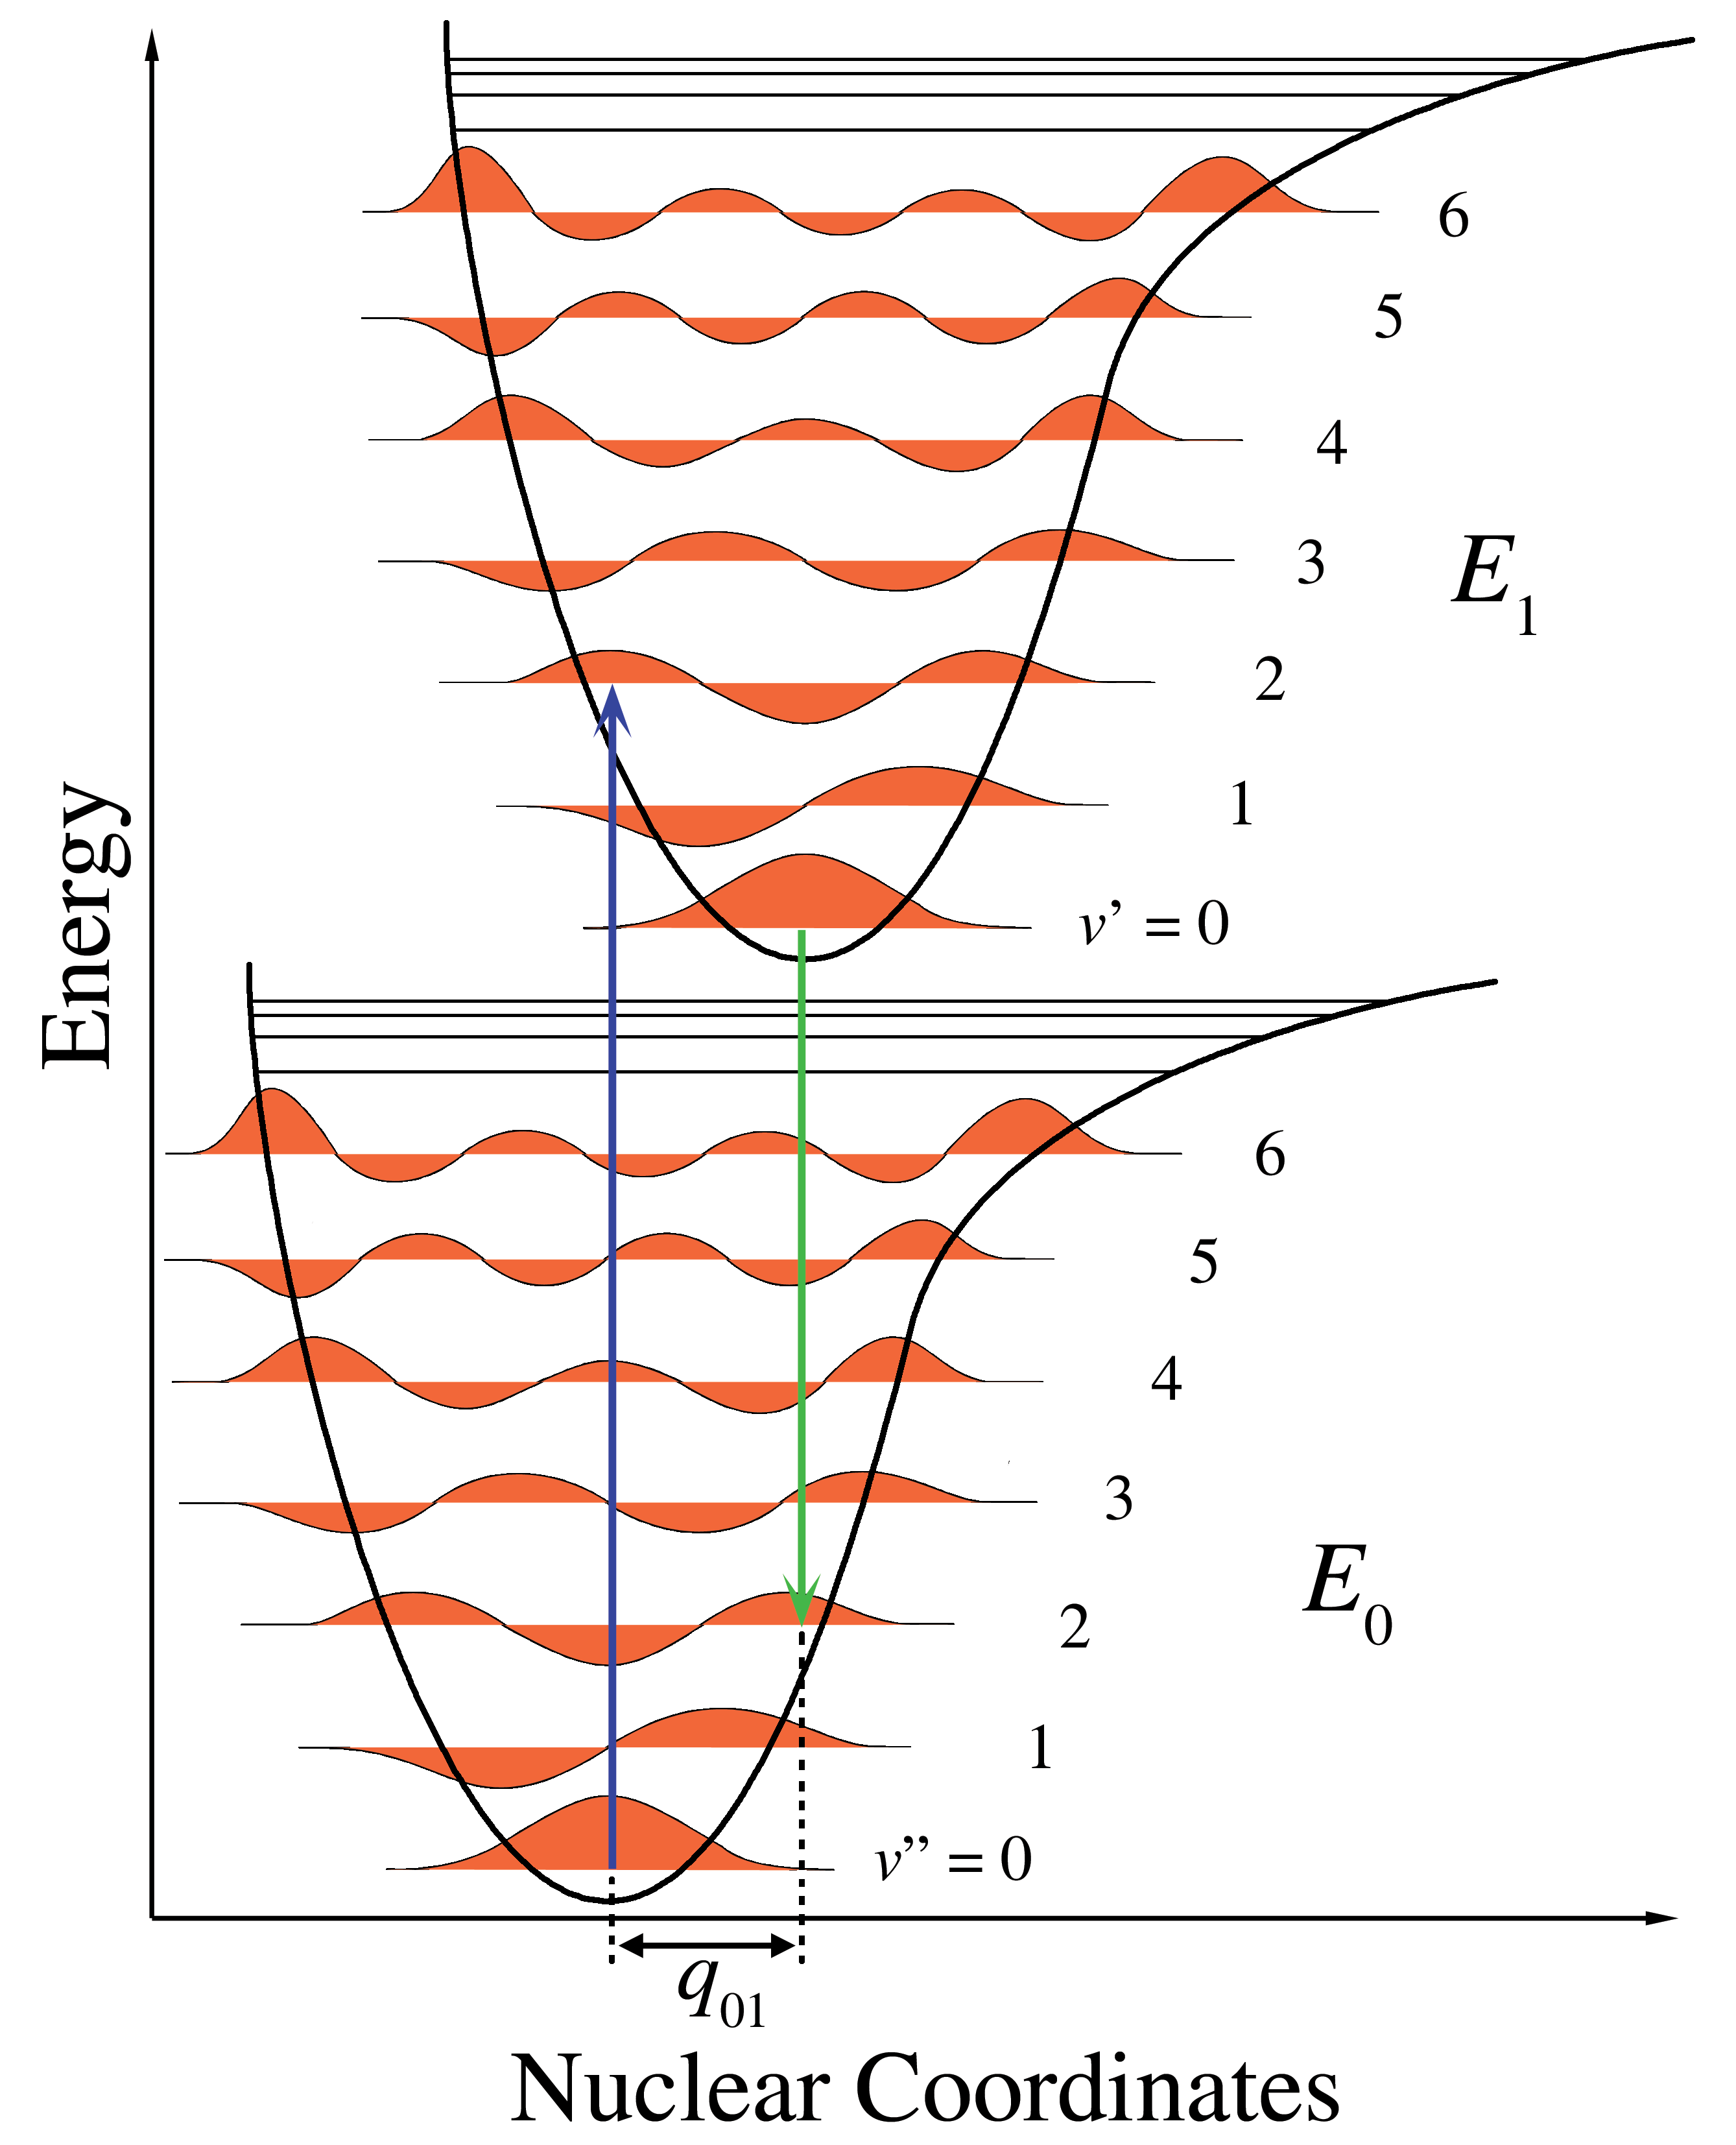
\includegraphics[width=0.5\linewidth]{img/condon.png}}
\hfill
\subfloat[][Spectrum]{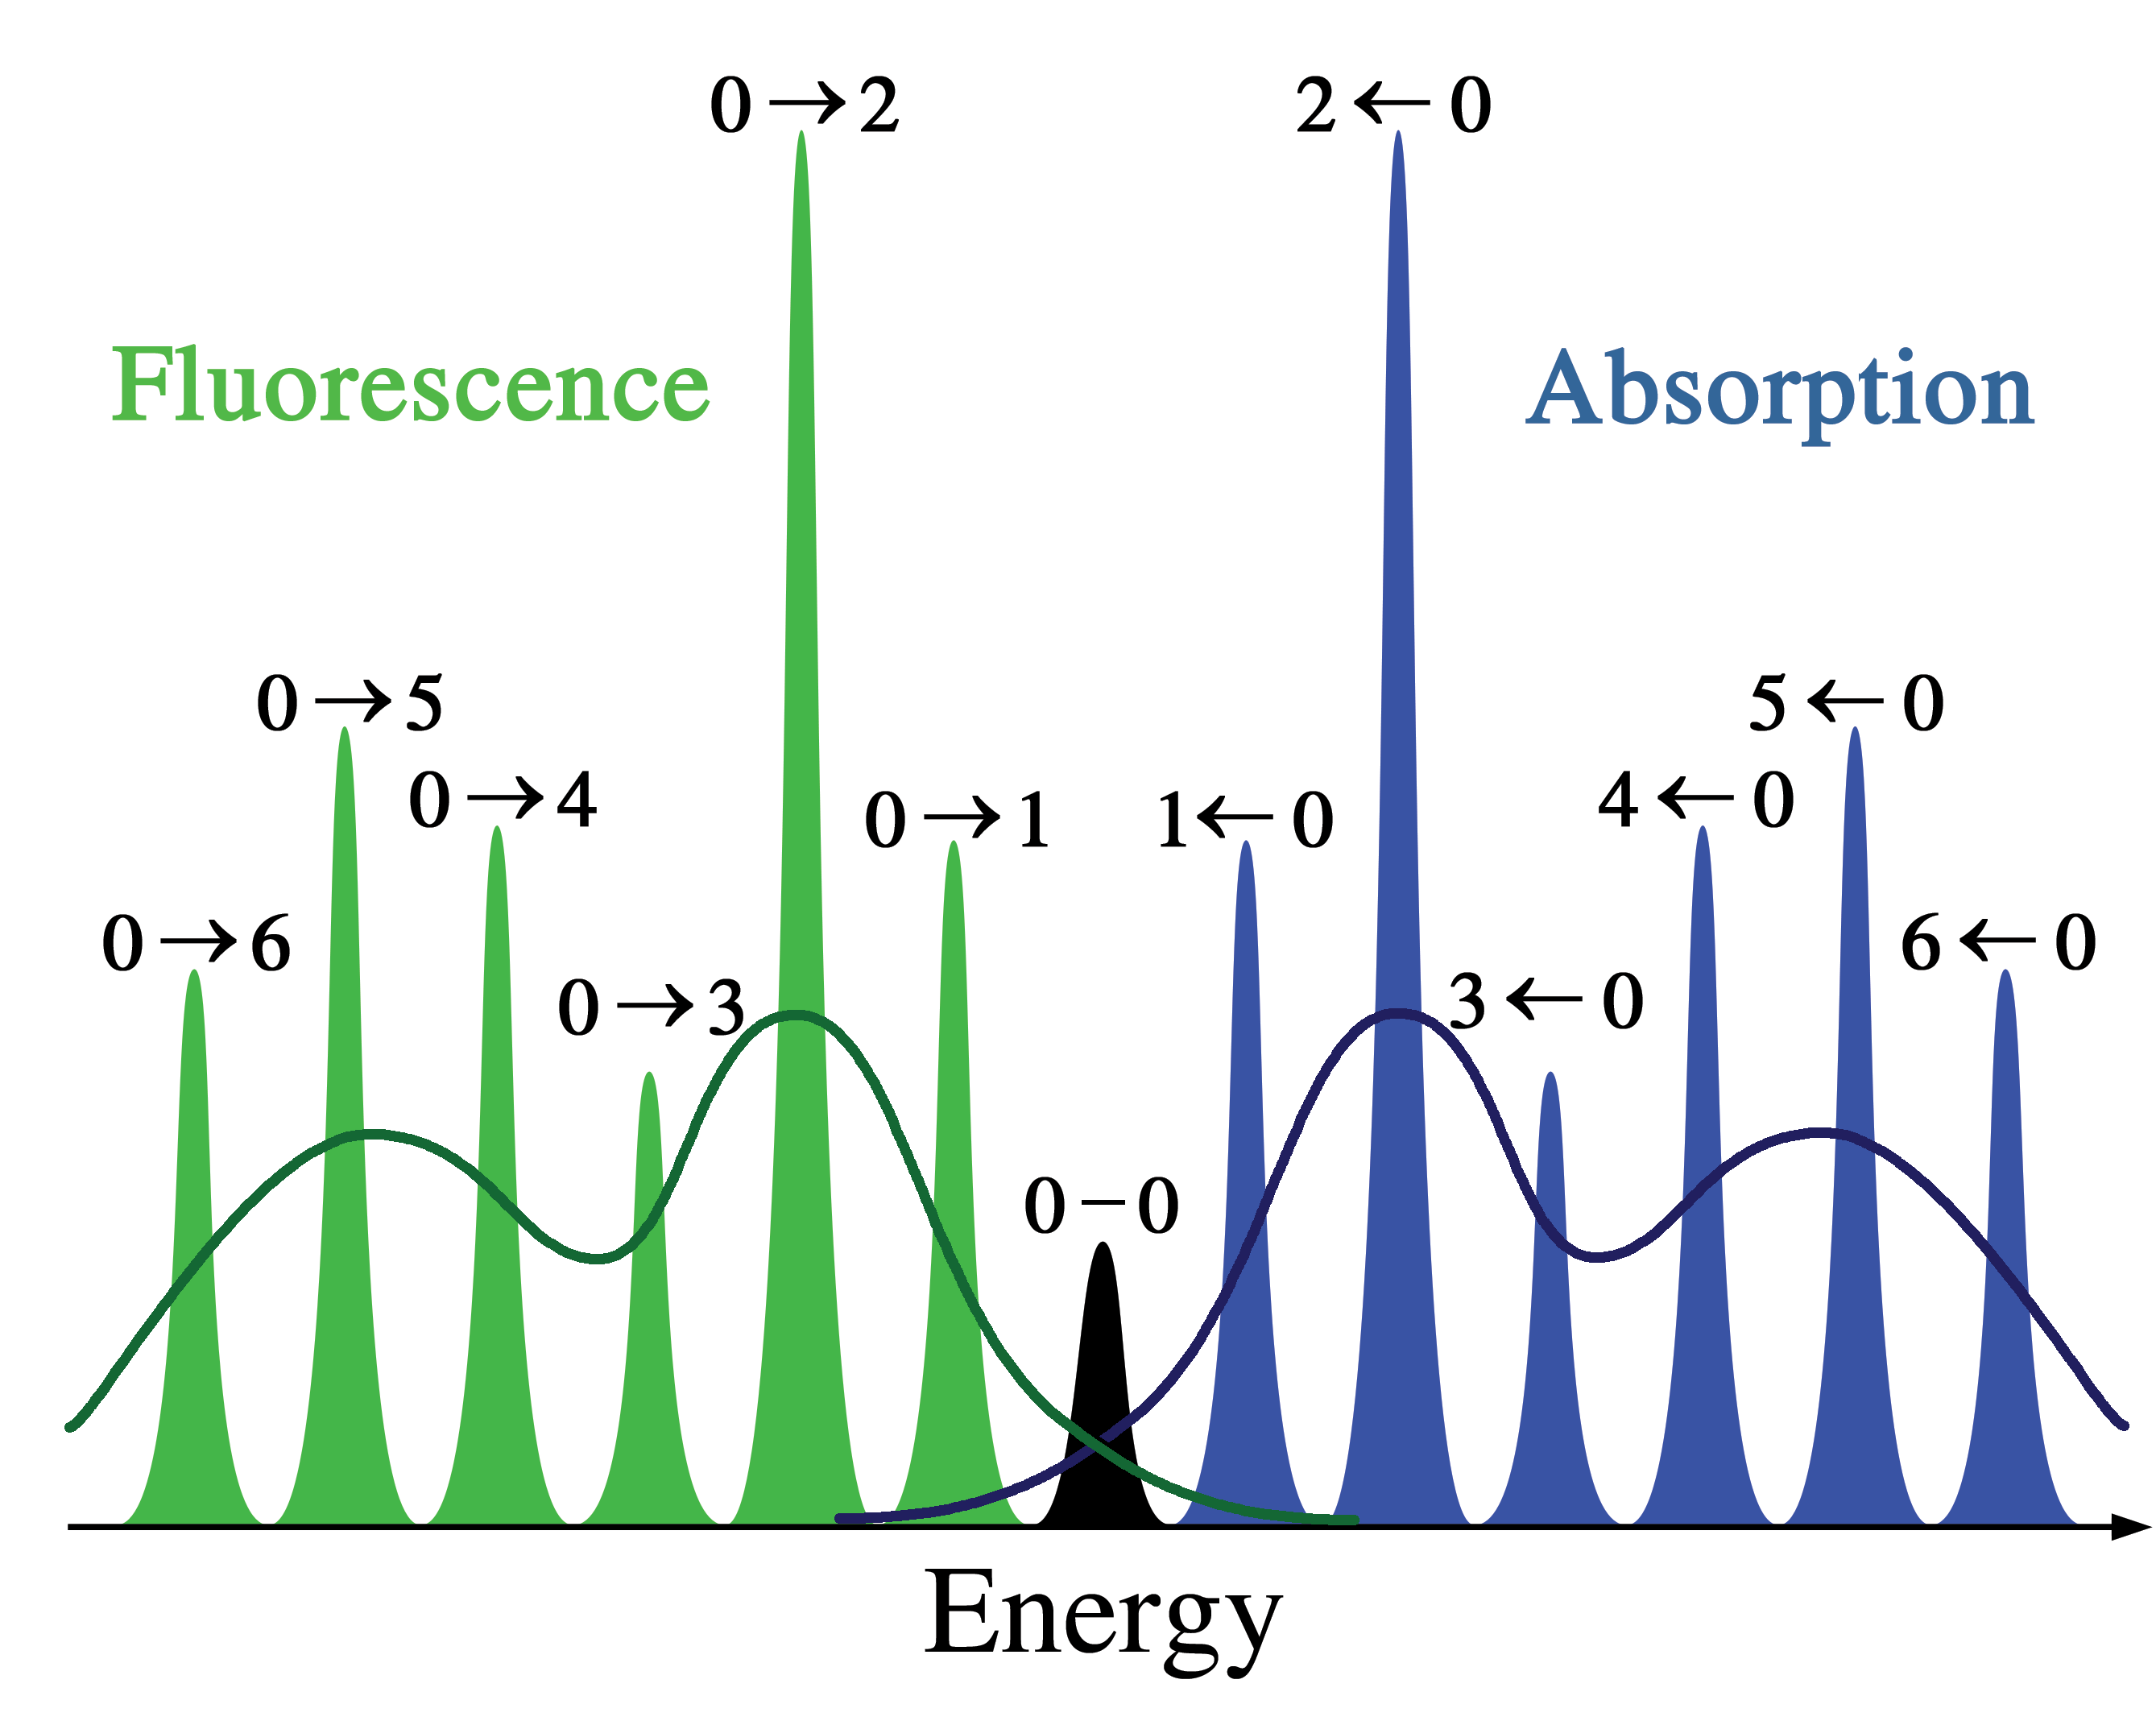
\includegraphics[width=0.5\linewidth]{img/absorptionemission.png}}

\subfloat[][Jablonski Diagram]{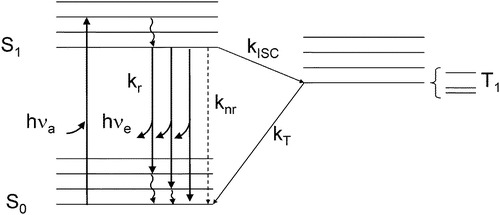
\includegraphics[width=0.7\textwidth]{img/Jablonski.jpg}}
\caption{ \small \textbf{(a)} Illustration of the Franck-Condon principle, which is a direct consequence of the Born-Oppenheimer approximation and states, that those electronic-vibraonic transitions are favored, which leave the inter-nuclei distance mostly unchanged. 
\textbf{(b)} Symmetric structure of an absorption and fluorescence spectrum. Sharp peaks will be visible in dilute gases, while in liquids and solids the peaks are widened. 
\textbf{(c)} Jablonski Diagram of different relaxation processes. ISC denotes intersystem crossing. $K_T$ the relaxation via phosphorescence. $K_r$ denotes fluorescence and $K_{nr}$ radiationless transitions, which also reduce the fluorescence lifetime. \footnotesize Source: \textbf{(a)}, \textbf{(b)} \url{http://en.wikipedia.org/wiki/Franck-Condon_principle}, \textbf{(c)} \cite{omg}}
\label{condon}
\end{figure}

\begin{figure}
\centering
\subfloat[][DPH Molecule]{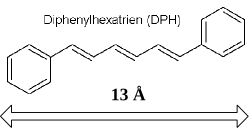
\includegraphics[width=0.5\linewidth]{img/dph.png}}
\subfloat[][Lipid Membrane]{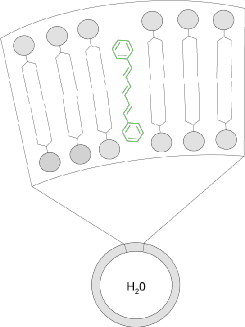
\includegraphics[width=0.35\linewidth]{img/membrane.png}}
\caption{ \small \textbf{(a)}Diphenylhexatriene (DPH) molecule, which is used as a reporter molecule in the lipid membrane. \textbf{(b)} Lipid membrane vesicle with a close-up of the bilayer, where a DPH molecule is embedded.}
\label{dph}
\end{figure}



\subsection{Rotational Diffusion}
After excitation with a polarized photon, the dipole moment is most probably aligned into the direction of the polarization. A photon emitted directly after excitation would than have the same polarization. However, as a certain time passes between excitation and radiative relaxation, the molecule can rotate in the mean time, which leads to a shift of the polarization. This rotational diffusion leads to the relaxation into an equilibrium state, which is completely isotropic unless certain symmetries are broken. The decay rate of this relaxation and the final state both give information about the degrees of freedom of the molecule and thus also about the environment of the molecule. A simple quantity to measure the rotational anisotropy is defined by
\eq{R=\frac{I_V -I_H}{I_V + 2I_H} \; ,}{R}
where $I_{V,H}$ denote the intensities of the fluorescence after excitation with a vertical or horizontal polarized beam. In a set-up, where also the polarization of the outgoing beam is measured, a more complex version of the rotational anisotropy is used \cite{lako}.
%wobbing cone


\subsection{Phase Transition}
Obviously the mobility of the membrane and thus the anisotropy is dependant on the temperature $T$. The plot of $R(T)$ is not a linear (or other simple) function though, but presents a steep change between two linear functions at a critical temperature $T_C$. This corresponds to a phase transition in the membrane between a phase of two dimensional liquid crystals and gel like phase.

To describe the steep change between the two phases further consider the equilibrium with particle numbers $M_1=M_2$. The equilibrium constant can be written as
\eq{K = \frac{M_2}{M_1} = K_0 e^{\frac{\delta H}{R T}}}{K}
\eq{\Rightarrow \frac{d}{dT}(\ln K) = \frac{\delta H}{R T}}{dK}
where $R$ is the universal gas constant and $\delta H$ the change in enthalpy. This last equation is called the van't Hoff equation. The degree of transformation 
\eq{\Theta = \frac{M_2}{M_1+M_2}}{Theta}
together with equation \ref{dK} allows for the determination of $\delta H$ in terms of the change of $\Theta$ at the critical temperature $T_C$ where $M_1=M_2$
\eq{{\left.\frac{d\Theta}{dT}\right |}_{T_C} = \frac{\delta H}{4 R T^2} .}{dTheta}

\clearpage

\section{Experiment}
\subsection{Absorption and Emission Spectra}
The emission and absorption spectrum of a sample with \SI{8}{\micro l} \SI{1}{mM} DPH in THF in \SI{1}{ml} vesicle solution (A) is analyzed and compared with a sample of the same DPH-THF solution, but dissolved in a buffer solution and not in a vesicle solution (B). The measurement is performed with a set-up displayed in figure \ref{fig:setup}. The absorption spectrum of sample A is measured for excitation wavelength between $\lambda_\text{ex}=\SI{270}{nm} - \SI{420}{nm}$ at a fixed emission wavelength of $\lambda_\text{em}=\SI{450}{nm}$. The polarization filters are switched to vertical polarization to achieve highest intensity. The resolution of the spectrum is set to $\Delta \lambda =\SI{6}{nm}$ and the photomultipliers  are operated at: PM1 (sample) Range \SI{300}{nA}, Voltage \SI{13}{V}; PM2 (reference) Range \SI{3}{\micro A}, Voltage \SI{13}{V}.

The emission spectrum for sample A and B are recorded at an excitation wavelength of $\lambda_\text{ex}=\SI{360}{nm}$ for emission wavelength $\lambda_\text{ex}=\SI{380}{nm} - \SI{530}{nm}$ at the same operation parameters for the photomultipliers and polarization, except for the range of photomultiplier 1 (sample) that is changed to \SI{300}{nA} for the measurement of sample B, because the low intensity.

\subsection{Steady State Fluorescence Depolarization}
In order to investigate the phase transition of DMPC, the anisotropy is measured at different temperatures. For each temperature and all four combinations of polarizations of the two polarizers 5 intensity values are recorded and the average value is used for the calculation of the anisotropy. As the temperature can only be measured before and after each measurement, the  values are plotted against the averaged temperature (before and after measurement).


\begin{figure}
\centering
\subfloat[][Static Set-Up]{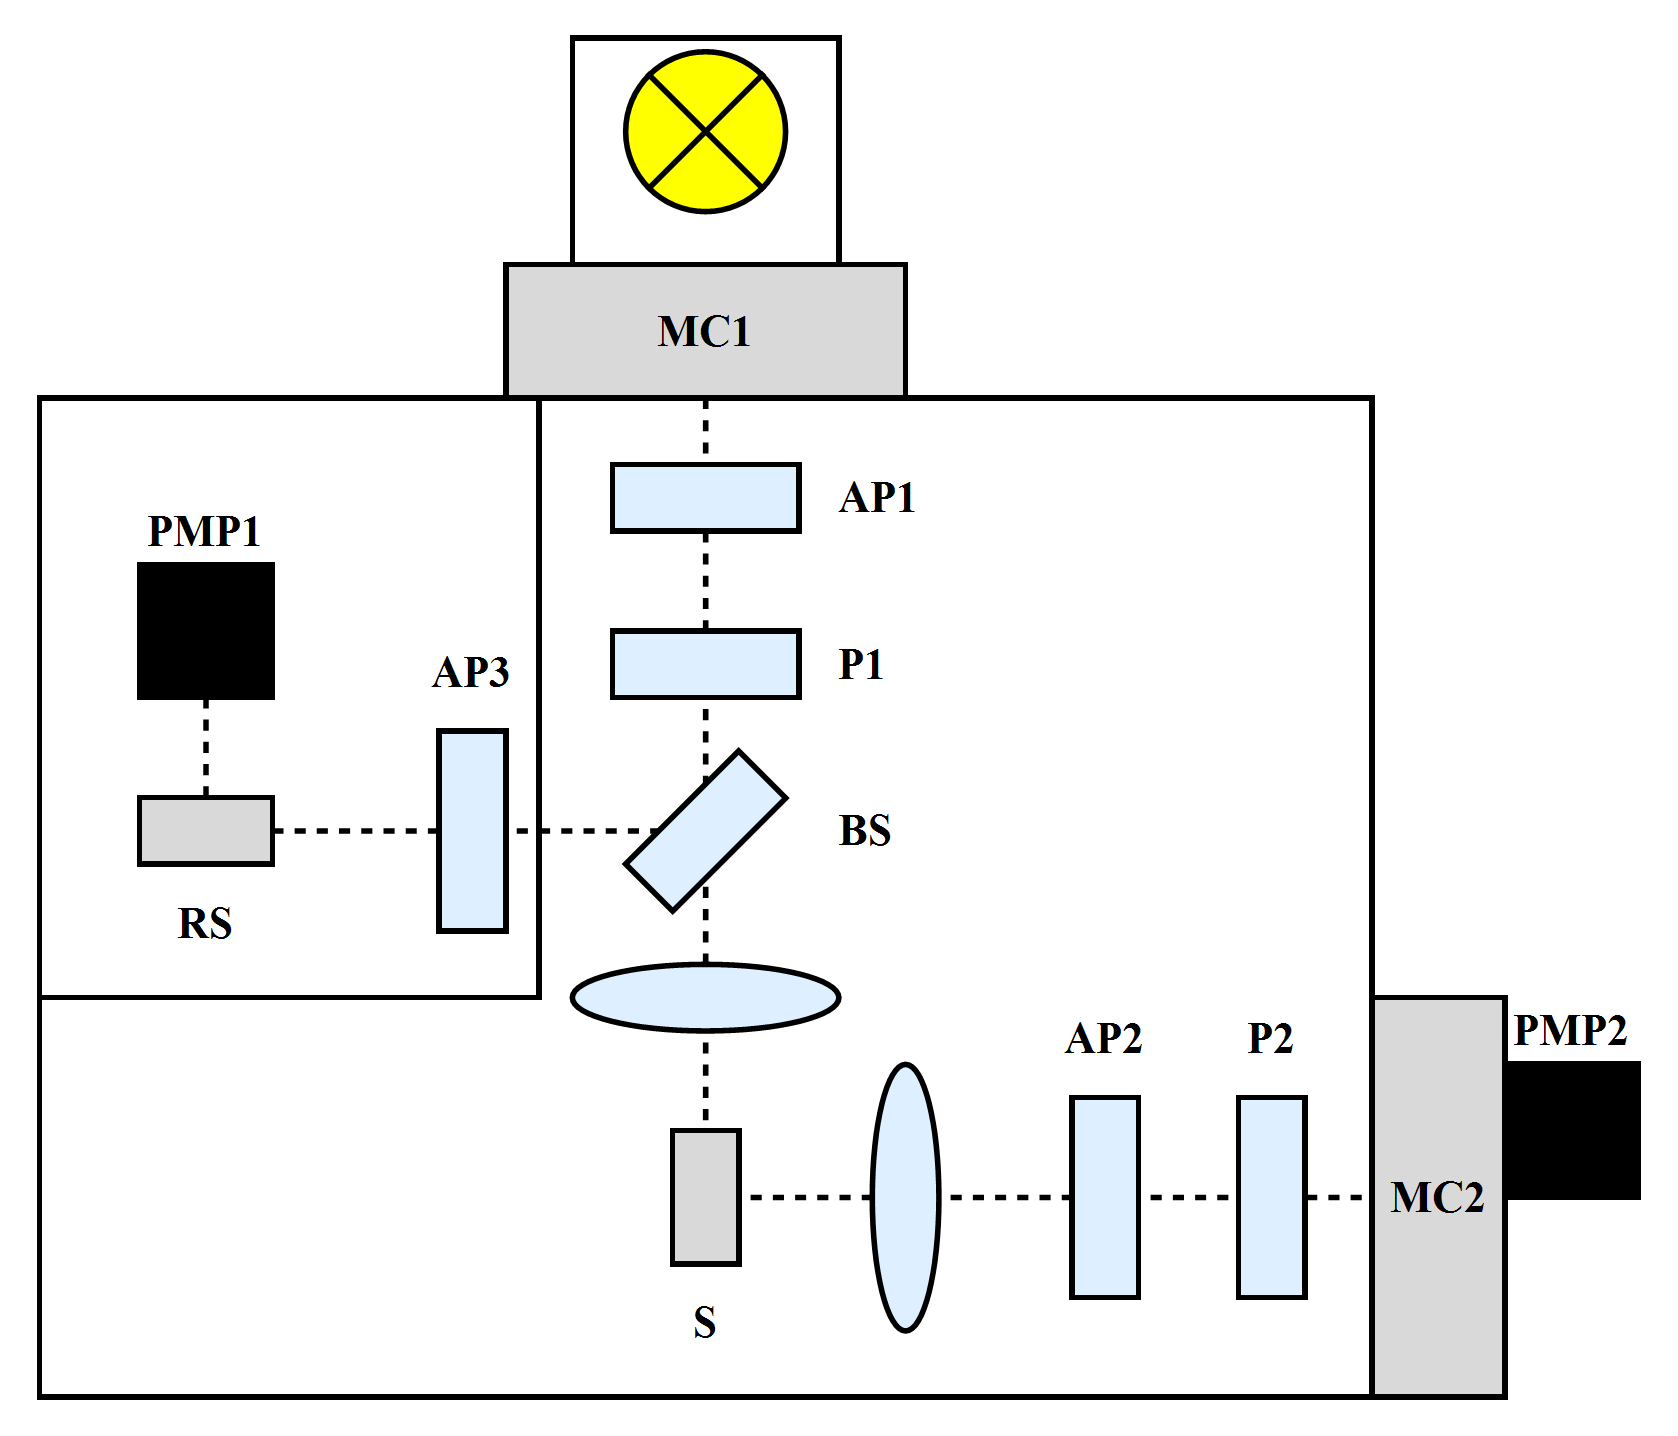
\includegraphics[width=0.55\linewidth]{img/setupStatic.png}}
\hfill
\subfloat[][Time Resolved Set-Up]{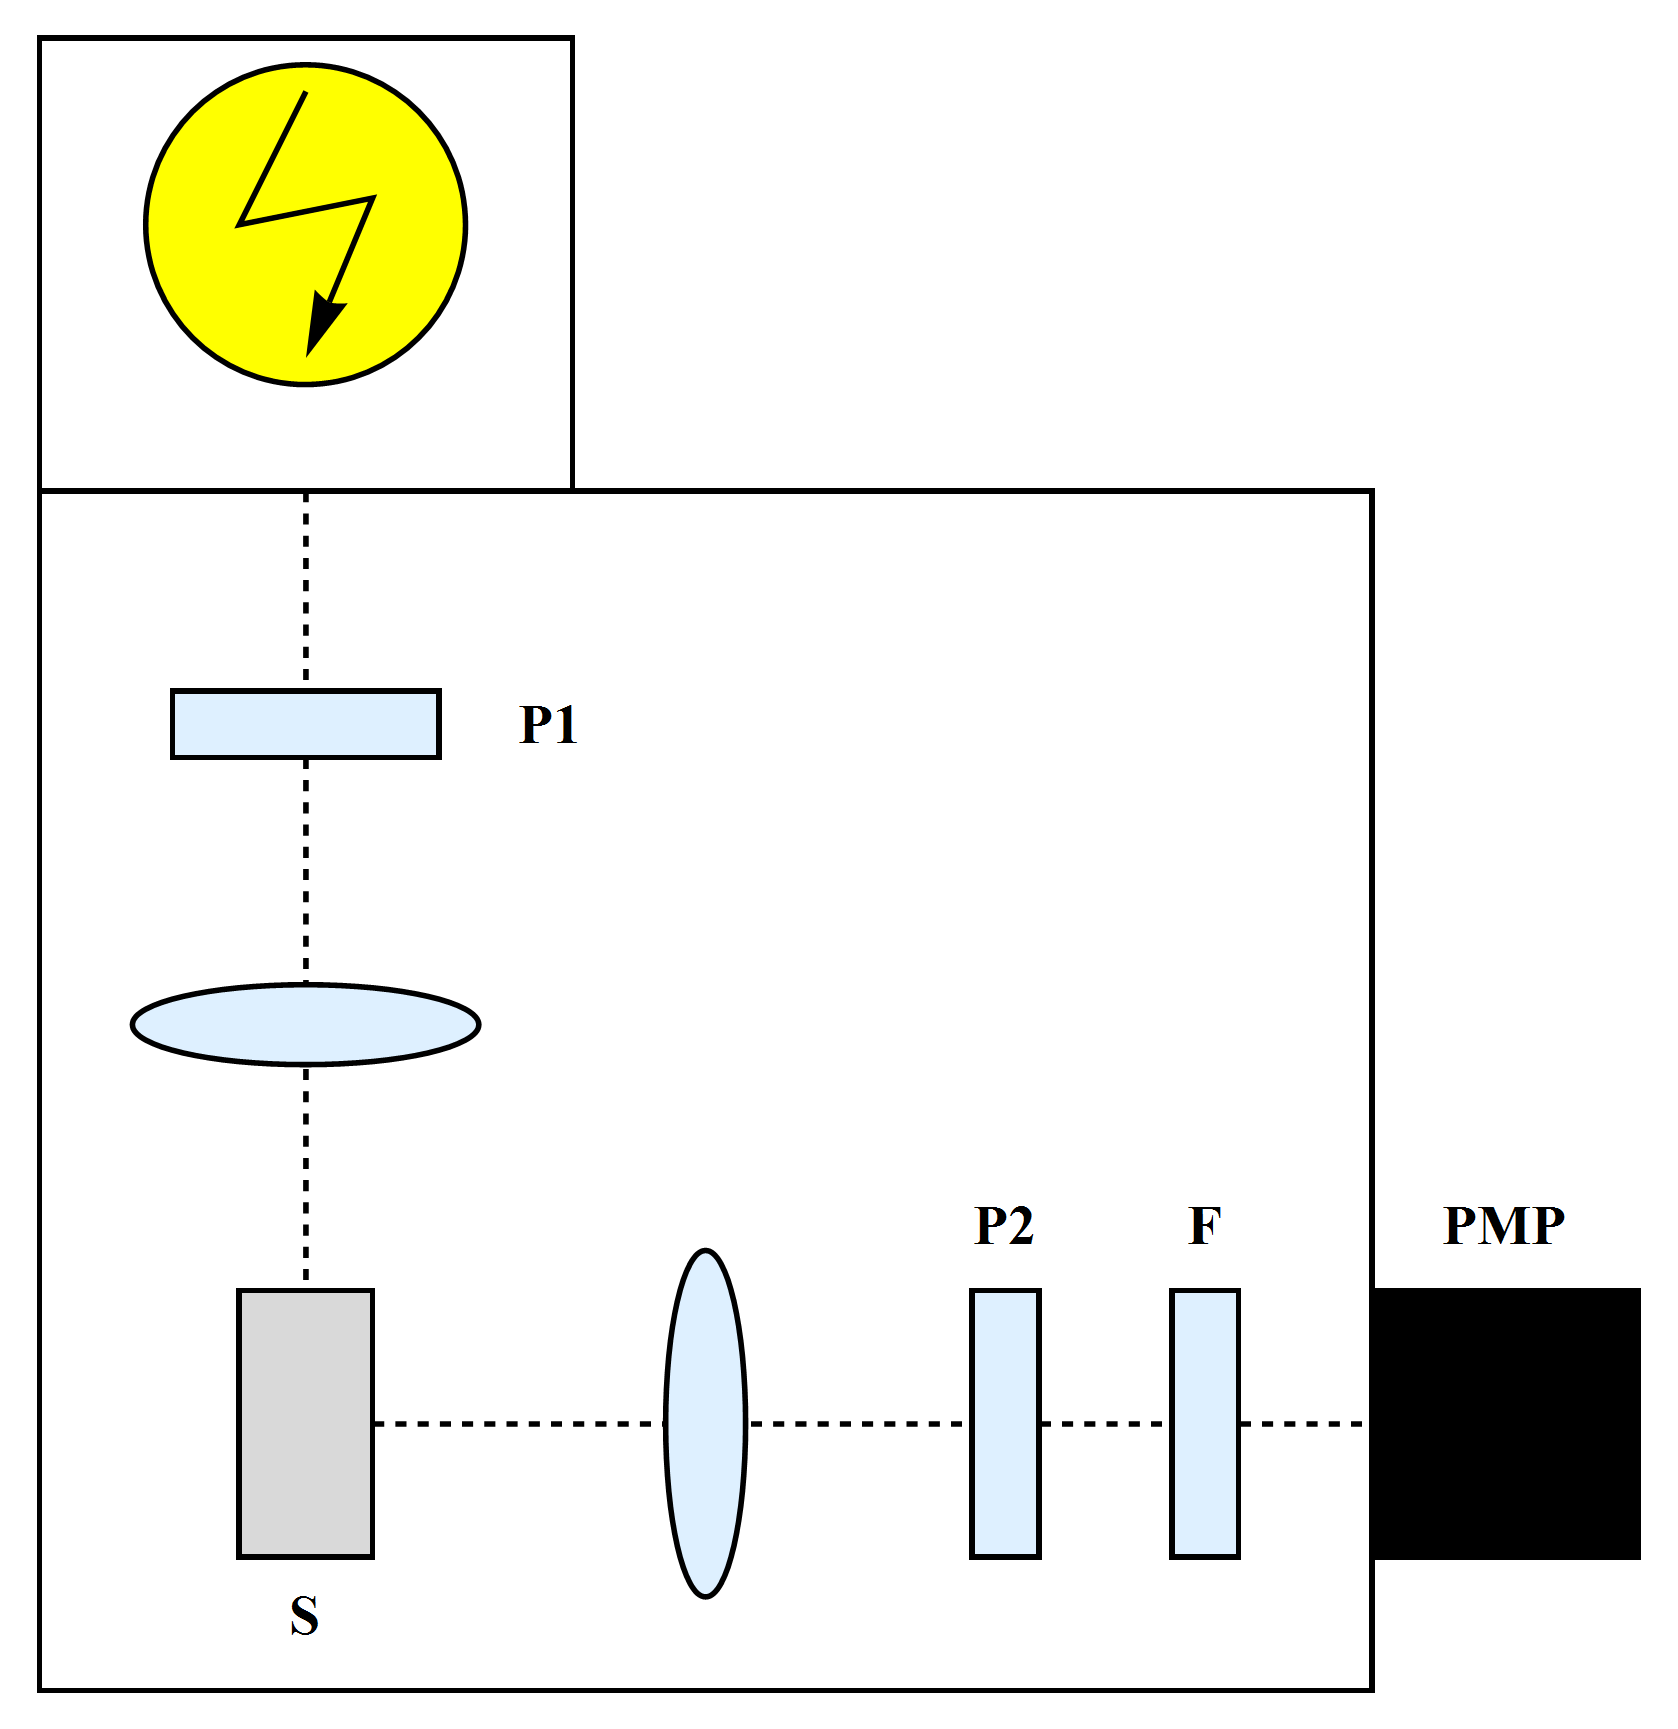
\includegraphics[width=0.45\linewidth]{img/setupDynamic.png}}
\caption{ \small \textbf{(a)} Set-Up for . \textbf{(b)} Set-Up for.}
\label{fig:setup}
\end{figure}

\clearpage

\section{Analysis}

\subsection{Phase Transition of DMPC}

\eq{I_\parallel = \frac{I_\text{VV}}{I_\text{HV}} , \qquad I_\perp = \frac{I_\text{VH}}{I_\text{HH}} \; . }{idef}
Slope left and right of the phase transition $s = (-1.4 \pm 0.4 ) \cdot 10^{-3} / \degree \text{C}$.
\eq{ T_C = ( 28.0 \pm 0.2 ) \, \degree \text{C} \; .}{Tc}

\begin{figure}
\centering
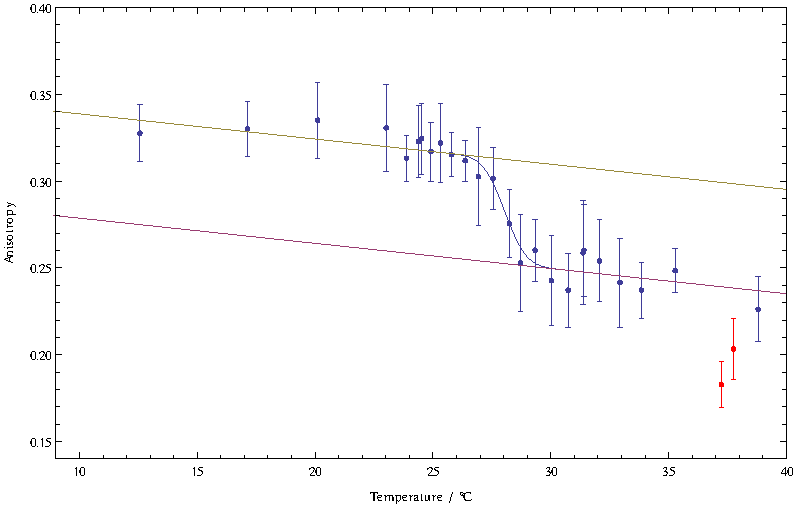
\includegraphics[width=\linewidth]{img/phasetransition.pdf}
\caption{ \small Fluorescence anisotropy of a vesicle membrane (DMPC lipids) for different temperatures. At $T_C=28.0 \, \degree$ C an abrupt change of the anisotropy indicates a phase transition. The points marked in red are considered to be outliers and are ignored in the fit.}
\label{fig:phase}
\end{figure}


\clearpage
 \bibliographystyle{unsrt}
\bibliography{bib}



\end{document}


